
\section*{Supplement}

\setcounter{figure}{0}
\makeatletter 
\renewcommand{\thefigure}{S\@arabic\c@figure}
\makeatother

\begin{figure}
  \begin{center}
    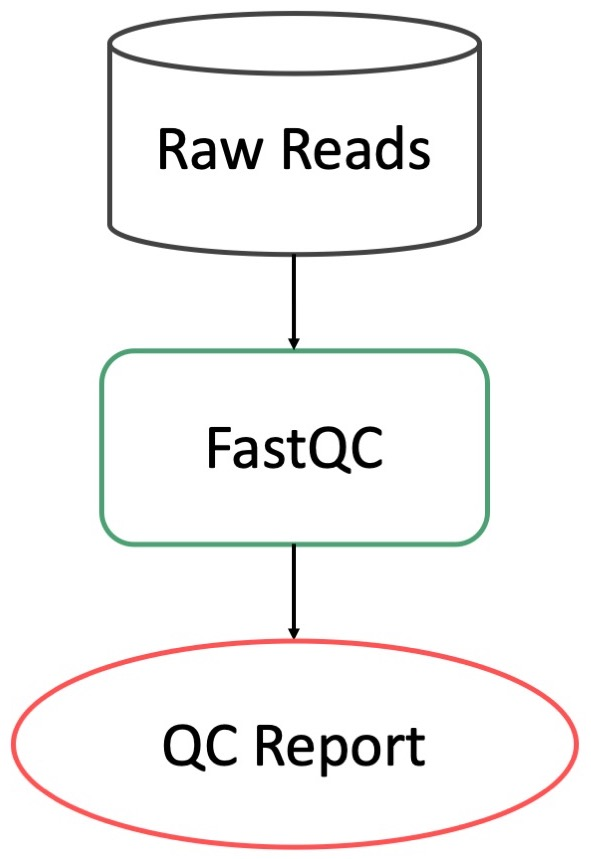
\includegraphics[width=0.4\textwidth]{figs/sfig_qc.jpeg}
%	\vspace{-20pt}
	\caption{\small{
	    Quality control stage, black cylinders represent raw data, orange ovals are results, and green boxes are tools.
	}}
    \label{fig:qc}
  \end{center}
%  \vspace{-20pt}
 % \vspace{1pt}
\end{figure}

\begin{figure}
  \begin{center}
    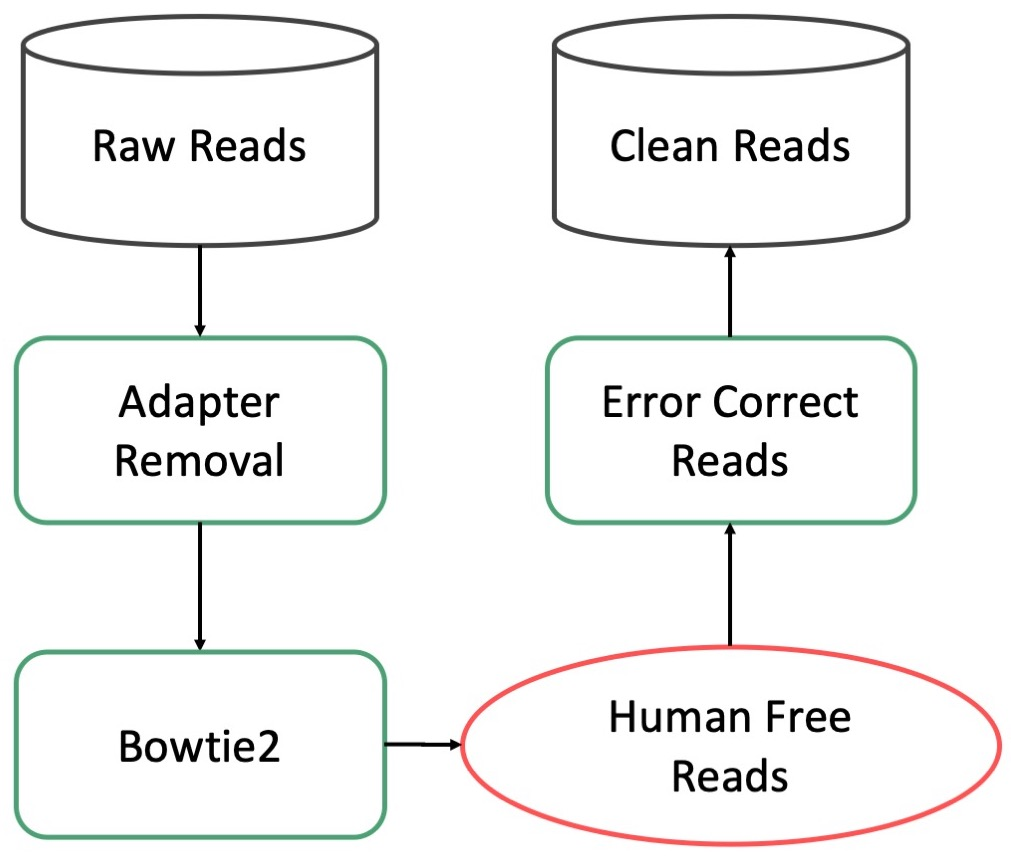
\includegraphics[width=0.8\textwidth]{figs/sfig_pre.jpeg}
%	\vspace{-20pt}
	\caption{\small{
	    Preprocessing stage, black cylinders represent raw data, orange ovals are results, and green boxes are tools.
	}}
    \label{fig:pre}
  \end{center}
%  \vspace{-20pt}
 % \vspace{1pt}
\end{figure}

\begin{figure}
  \begin{center}
    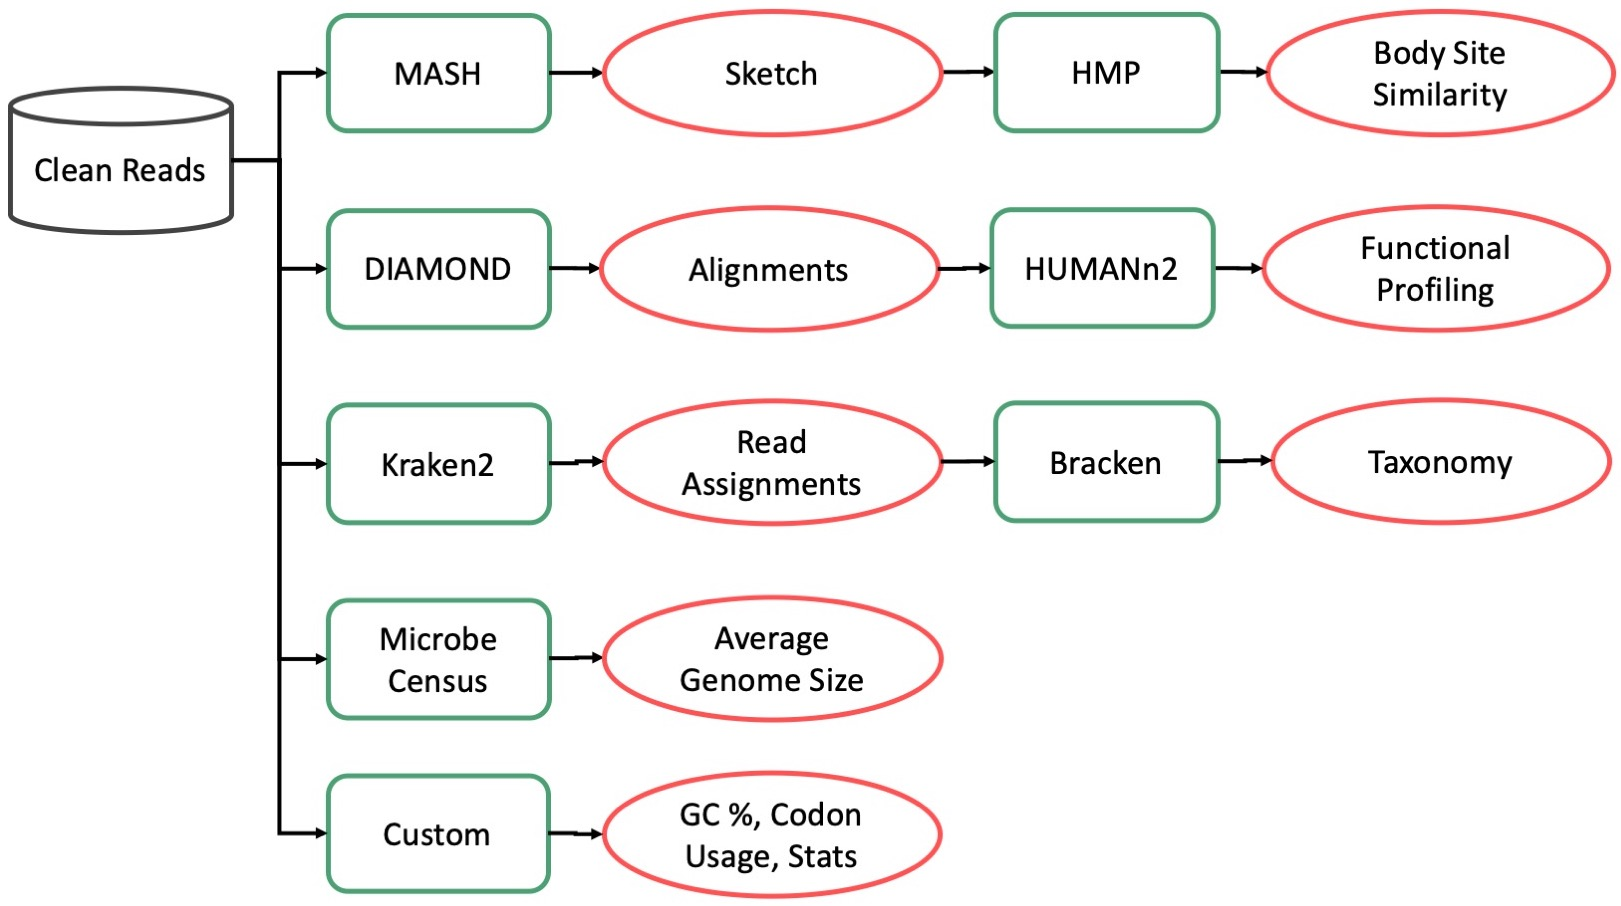
\includegraphics[width=0.95\textwidth]{figs/sfig_sr.jpeg}
%	\vspace{-20pt}
	\caption{\small{
	    Short Read stage, black cylinders represent raw data, orange ovals are results, and green boxes are tools.
	}}
    \label{fig:sr}
  \end{center}
%  \vspace{-20pt}
 % \vspace{1pt}
\end{figure}

\begin{figure}
  \begin{center}
    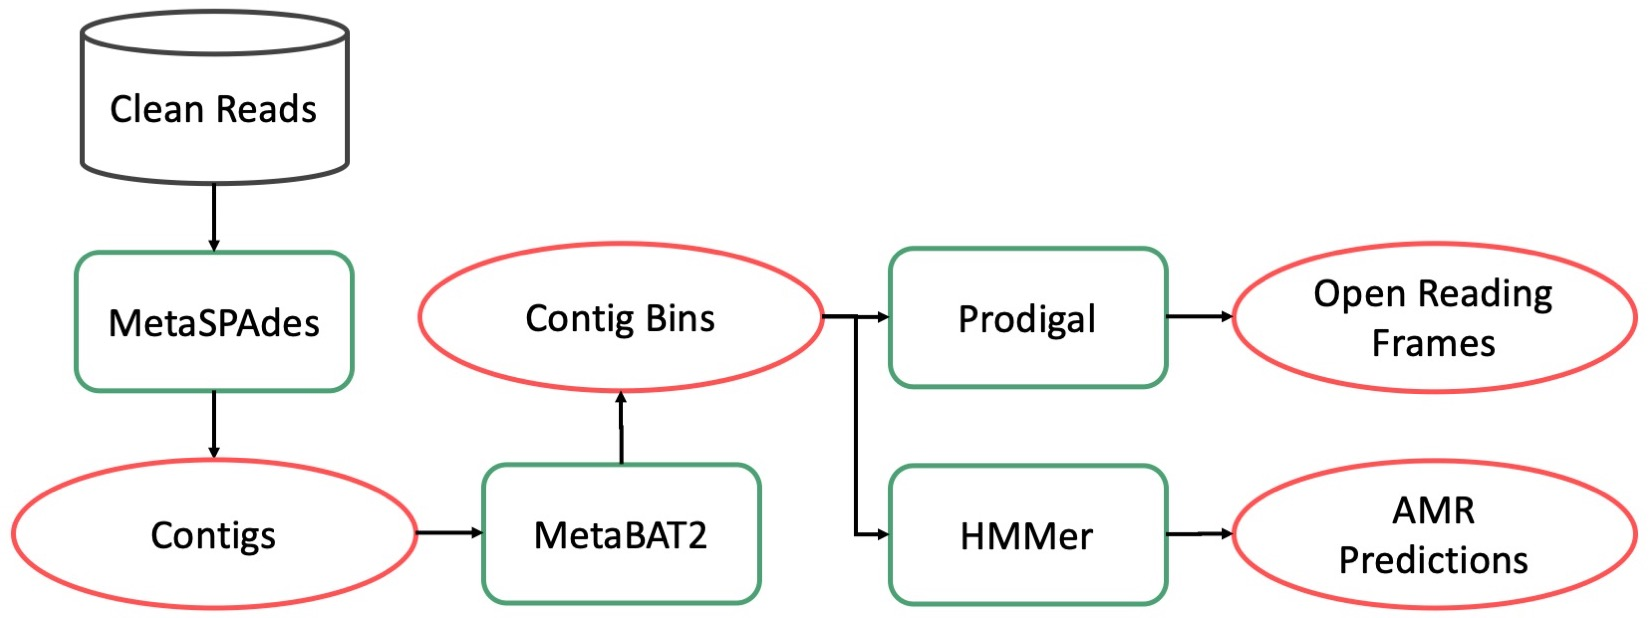
\includegraphics[width=0.95\textwidth]{figs/sfig_assembly.jpeg}
%	\vspace{-20pt}
	\caption{\small{
	    Assembly stage, black cylinders represent raw data, orange ovals are results, and green boxes are tools.
	}}
    \label{fig:assembly}
  \end{center}
%  \vspace{-20pt}
 % \vspace{1pt}
\end{figure}

\begin{figure}
  \begin{center}
    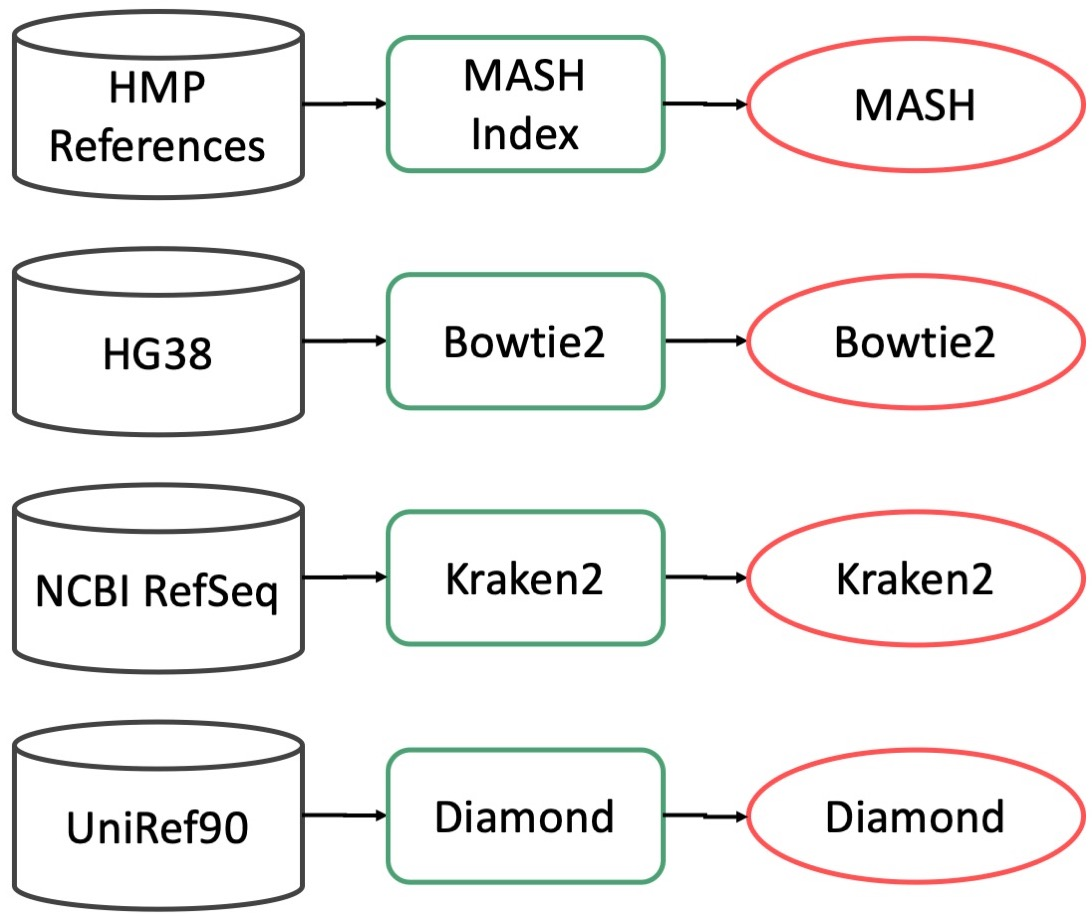
\includegraphics[width=0.8\textwidth]{figs/sfig_db.jpeg}
%	\vspace{-20pt}
	\caption{\small{
	    Database stage, black cylinders represent raw data, orange ovals are results, and green boxes are tools.
	}}
    \label{fig:db}
  \end{center}
%  \vspace{-20pt}
 % \vspace{1pt}
\end{figure}